\chapter{Simulation of an Ideal Gas}

\section{Introduction}

For an ideal gas composed of molecules with mass $m$ at temperature
$T$, the probability density for the component of velocity in the $x$
direction ($v_x$) is given by:
\begin{equation}
  \label{eqn:mbvx}
P(v_x) = \sqrt{\frac{m}{2 \pi k_{\rm B} T}} \exp\left(-\frac{m v_x^2}{2k_{\rm B} T}\right)
\end{equation}
where $k_{\rm B}$ is Boltzmann's constant.  Similary for the $y$ direction:
\begin{equation}
  \label{eqn:mbvx}
P(v_y) = \sqrt{\frac{m}{2 \pi k_{\rm B} T}} \exp\left(-\frac{m v_y^2}{2k_{\rm B} T}\right).
\end{equation}

For simplicity, we will be simulating a gas in two dimensions.  The infinitesimal probability associated with a velocity $(v_x, v_y)$ is given by: 
\begin{eqnarray*}
P(v_x, v_y) \, dv_x \, dv_y &=& P(v_x) \, dv_x \, P(v_y) \, dv_y \\
   &=& \frac{m}{2 \pi k_{\rm B} T} \exp\left(-\frac{m (v_x^2+v_y^2)}{2k_{\rm B} T}\right) \, dv_x \, dv_y \\
   &=& \frac{m v}{2 \pi k_{\rm B} T} \exp\left(-\frac{m v^2}{2k_{\rm B} T}\right) \, d\theta \, dv \\
\end{eqnarray*}
where we have changed to polar coordinates $v$ and $\theta$ in the usual manner with area differential $dv_x \, dv_y = v \, dv \, d\theta$.  This allows us to read off the probability density in polar coordintes:
\begin{equation*}
P(v, \theta) = \frac{m v}{2 \pi k_{\rm B} T} \exp\left(-\frac{m v^2}{2k_{\rm B} T}\right) 
\end{equation*}
Integrating over all possible directions $\theta$, we obtain:
\begin{eqnarray}
P(v) &=& \int_0^{2\pi} P(v,\theta) d\theta \nonumber \\
     &=& \int_0^{2\pi} \frac{m v}{2 \pi k_{\rm B} T} \exp\left(-\frac{m v^2}{2k_{\rm B} T}\right) \nonumber \\
P(v) &=& \frac{m v}{k_{\rm B} T} \exp \left(-\frac{m v^2}{2k_{\rm B} T}\right) \label{eqn:mbv}\\
\nonumber
\end{eqnarray}
which is the Maxwell-Boltzmann distribution for an ideal gas in two
dimensions.  This is the probability density for a gas molecule to have speed
$v$.

In this lab, we will create a simple numerical simulation of an ideal
gas and verify that the velocity of the gas follows the
Maxwell-Boltzmann distribution.

\section{System of Units}

Choosing an effective system of units is essential for building a
well-behaved numerical simulation.  Consider the Maxwell-Boltzmann
distribution, which involves the following SI values:
\begin{itemize}
\item Boltzmann's constant: $k_{\rm B} = 1.38 \times 10^{-23}~\rm J/K$
\item Molecular masses: e.g. $N_2$ with $m =  4.65 \times 10^{-26}~ \rm kg$.
\item Temperature: e.g. room temperature $T = 293~\rm K$.
\end{itemize}
The smallest number greater than zero that a computer can represent
with a single-precision floating point number is approximately
$10^{-38}$. Representing the SI value of Boltzmann's constant at
$10^{-23}$ uses a large fraction of this precision before we even begin
our calculation.  Numerical algorithms using floating point numbers
work best when the values involved in the calculation are near one.

It is usually best, therefore, to devise an alternate system of units
for any numerical simulation which keeps the values of variables of
interest as near one as possible.  We will call this the numerical
system of units.

To start, we choose a reference temperature near the temperature
we would like to simluate, say $T_0 = 293~\rm K$.  All temperatures in
the simulation will be in units of this reference temperature.  So a
temperature {\tt T=1.2} in the program will be $1.2 \, T_0 = 352~\rm K$
in SI units.  Our model also includes mass, so we choose a reference
mass near the mass of the molecules we will be simulating, say $M_0 =
4.65 \times 10^{-26}~ \rm kg$.  A mass {\tt m=2.1} in our program would have
an SI value value of $2.1 M_0 = 9.8 \times 10^{-26}~ \rm kg$.

The physics we will simulate involves Boltzmann's constant $k_{\rm B}$
which will have a value of one in our program.  This sets the
reference energy from our reference temeperature.  For example, an
energy {\tt kT = 3} in our program will have an SI value of $k_{\rm B}
T = 3~k_B T_0 = 1.21 \times 10^{-20}~J$.  The reference energy and
reference mass together define a reference velocity:
\begin{displaymath}
V_0 = \sqrt{\frac{k_b T_0}{M_0}} = 295~ \rm m/s.  
\end{displaymath}  

The only time the actual values choosen for the numerical system of
units are needed is if you need to convert inputs in SI units to the
numerical system of units, or convert the results of your simulation
to SI units.  In this lab, we will specify all inputs and report all
results using the numerical system of units.  {\bf So there is no need for
specific values such as $M_0 = 2.32 \times 10^{-25}~\rm kg$ to appear
anywhere in your program.}  If such values do appear, outside of
comments, you are certainly making a mistake!

\begin{figure}[htbp]
\begin{center}
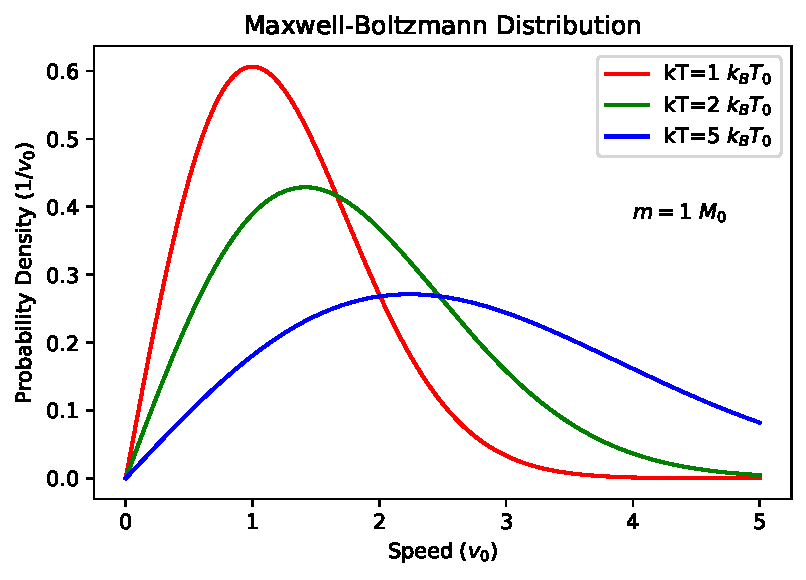
\includegraphics[width=0.65\textwidth]{figs/maxwellboltzman/maxboltz.pdf} \\
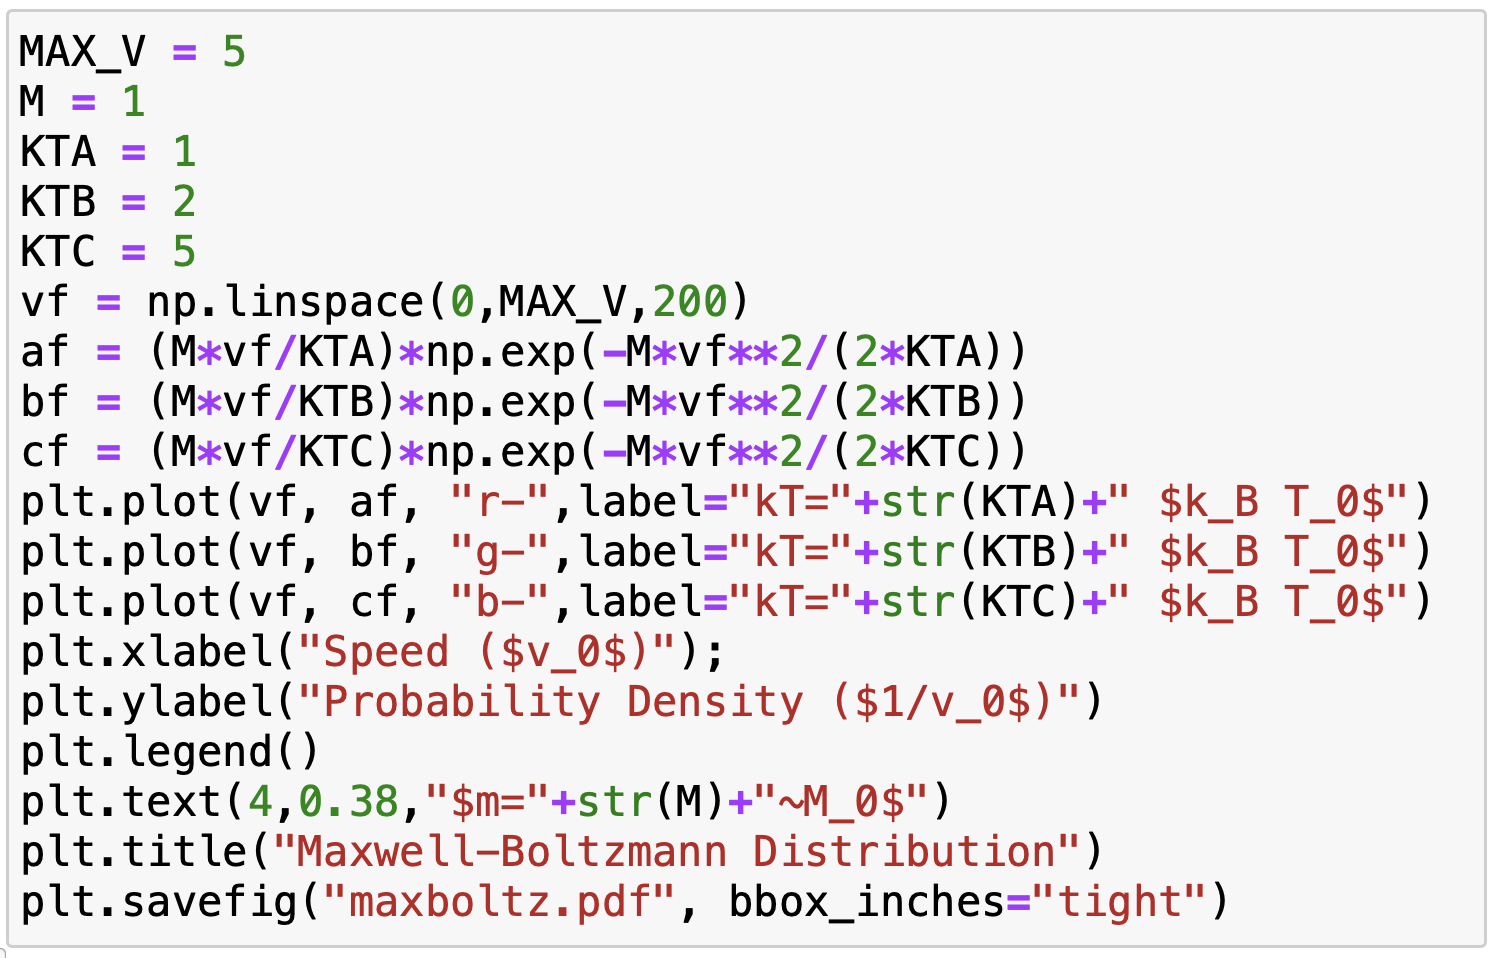
\includegraphics[width=0.65\textwidth]{figs/maxwellboltzman/maxboltz-code.png} \\
\caption{The Maxwell-Boltzmann distribution using a system of units appropriate for a numerical simulation, along with the code used to produce the plot.}
\label{fig:mbdist}
\end{center}
\end{figure}

As an example, the Maxwell-Boltzmann distribution is plotted in
Fig.~\ref{fig:mbdist} alongside the code used to produce it.  Notice
how for {\tt kT} and {\tt m} near one, the typical velcities are also
near one.  This is sign of good numerical system of units.  Notice
also that Boltzmann's constant or any other small or large numbers in
SI units do not appear anywhere in the code. 

\section{Collision Model}

At the heart of your numerical simulation is the collision model.  It
is the collisions of molecules that will allow your simulated gas to
reach thermal equilibrium.  We will use the simple elastic collision
of identical mass particles, as illustrated in Fig.~\ref{fig:collcms}, as our collision model.  We consider particles a and b with velocities $\vec{v_a}$ and
$\vec{v_b}$ in the lab frame.  The velocity of particle a in the CMS frame before the collision is
\begin{displaymath}
\vec{u} = \frac{\vec{v_a} - \vec{v_b}}{2}.
\end{displaymath}
The collision rotates the velocity of particle a by the scattering angle $\theta$ so that the velocity $\vec{w}$ after the collision is
\begin{displaymath}
\begin{pmatrix}
w_x \\
w_y \\
\end{pmatrix}
  =
\begin{pmatrix}
\cos \theta  & \sin \theta \\
-\sin \theta  & \cos \theta \\
\end{pmatrix}
\,
\begin{pmatrix}
u_x \\
u_y \\
\end{pmatrix}
\end{displaymath}
In the lab frame, the velocity of molecule a changes by an amount:
\begin{displaymath}
\Delta \vec{v_a} = \vec{w} - \vec{u}
\end{displaymath}
and the velocity of molecule b changes by an amount:
\begin{displaymath}
\Delta \vec{v_b} = \vec{u} - \vec{w}
\end{displaymath}




\begin{figure}[htbp]
\begin{center}
\begin{tikzpicture}
\draw[->, line width=1.5, blue] (-3,0) -- (-0.1,0);
\draw[->, line width=1.5, blue] (3,0)  -- (0.1,0);
\draw[->, line width=1.5, red] (0,0) -- (3*0.50,3*0.86) coordinate(A);
\draw[->, line width=1.5, red] (0,0) -- (-3*0.50,-3*0.86) coordinate(B);
\node[right] at (0.5,0.5) {$\theta$};
\node[left] at (-3,0) {a};
\node[right] at (3,0) {b};
\node[above] at (A) {a};
\node[below] at (B) {b};
\node[above] at (-1.5,0) {$\vec{u}$};
\node[above] at (1.5,0) {$-\vec{u}$};
\node[left] at (0.8,1.5) {$\vec{w}$};
\node[left] at (-0.8,-1.4) {$-\vec{w}$};
\end{tikzpicture}
\caption{The collision model in the center-of-mass:  incoming molecule $a$ with velocity $\vec{u}$ collides with the incoming particle $b$ of identical mass with velocity $-\vec{u}$.  Particle $a$ is scattered by angle $\theta$ and leaves with velocity $\vec{w}$, while particle $b$ leaves with velocity $\vec{w}$.  The magnitude of the final and initial velocities are the same:  $|\vec{u}| = |\vec{w}|$.}
\label{fig:collcms}
\end{center}
\end{figure}

\section{Implementing the Collision Model}

Our Python implementation for the collision will be computed in terms
of the components of the velocity vectors of molecule a and molecule
b:
\begin{eqnarray*}
\vec{v_a} &=& 
\begin{pmatrix}
a_x \\
a_y \\
\end{pmatrix} \\
\vec{v_b} &=& 
\begin{pmatrix}
b_x \\
b_y \\
\end{pmatrix} \\
\end{eqnarray*}
We'll use the Python variable names {\tt ax}, {\tt ay}, {\tt bx}, and {\tt by} to refer to $a_x$,  $a_y$,  $b_x$, and $b_y$.  

First calculate the $x$ and $y$ component of $\vec{u}$ as:
\begin{eqnarray*}
u_x &\equiv& \frac{a_x - b_x}{2} \\
u_y &\equiv& \frac{a_y - b_y}{2} \\
\end{eqnarray*}
Then compute the $x$ and $y$ component to the change in velocity of particle a and particle b:
\begin{eqnarray*}
  \Delta a_x &=& (\cos\theta - 1) \, u_x + \sin\theta \, u_y \\
  \Delta a_y &=& (\cos\theta - 1) \, u_y - \sin\theta \,  u_x \\
  \Delta b_x &=& (1-\cos\theta) \, u_x - \sin\theta \, u_y \\
  \Delta b_y &=& (1-\cos\theta) \, u_y + \sin\theta \,  u_x \\
\end{eqnarray*}
Finally, update the $x$ and $y$ components of the particle velocities to their value after the collision:
\begin{eqnarray*}
  a_x &\to& a_x + \Delta a_x \\
  a_y &\to& a_y + \Delta a_y \\
  b_x &\to& b_x + \Delta b_x \\
  b_y &\to& b_y + \Delta b_y \\
\end{eqnarray*}

In essential technique for programming complicated task is dividing
complicated tasks into smaller tasks, and thoroughly testing the
smaller tasks.  You cannot program effectively until you master this
technique.  I've taught students programming for many years, and the
students that finish last are invariably the ones that rush to
complete their entire program and then try to test and debug it.  This
approach always fails because when you do not get the right answer,
and you won't, ever, on the first try, you have absolutely no idea
what part of a very long chain of calculations is not programmed
correctly.

\begin{figure}[htbp]
\begin{center}
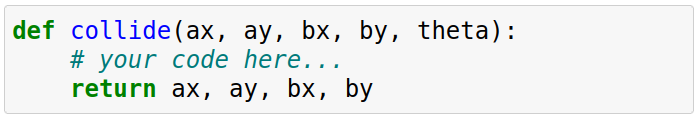
\includegraphics[width=0.65\textwidth]{figs/maxwellboltzman/collide.png} \\
\caption{Collision function.}
\label{fig:collfunc}
\end{center}
\end{figure}


To use this approach in the lab, we'll be implementing the collision
algorithm as a function, exactly as in Fig.~\ref{fig:collfunc}.  This
function takes as input the velocity components {\tt ax}, {\tt ay},
{\tt bx}, {\tt by} as defined above plus the scattering angle {\tt
  theta}.  In Fig.~\ref{fig:collfunc}, the function simply returns the
velocity components unchanged.  You should modify the function to
implement the scattering algoirthm described above.

Normally at this point, you would have to devise your own test to
validate your code.  One technique, that would work here, is to
calculate a few examples and then compare your program output to what
you obtained with paper and pencil.  For this lab, I will provide some
specific example calculations for you to validate your collision function.

\begin{figure}[htbp]
\begin{center}
  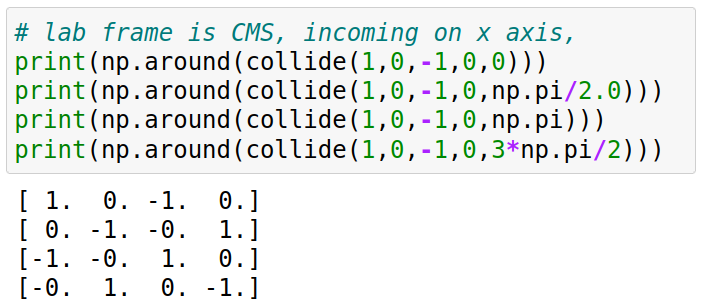
\includegraphics[width=0.65\textwidth]{figs/maxwellboltzman/collx.png} \\
  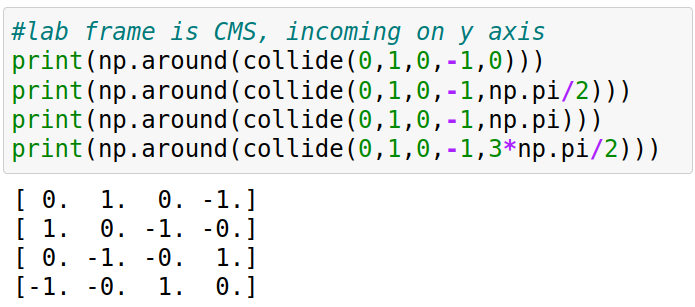
\includegraphics[width=0.65\textwidth]{figs/maxwellboltzman/colly.png} \\
  \caption{Example collisions along the $x$ and $y$ axis.}
\label{fig:collxy}
\end{center}
\end{figure}

\begin{plot} \end{plot}  Implement the collision algorithm as a function as in Fig.~\ref{fig:collfunc} and test it using example collisions from Fig.~\ref{fig:collxy}.

When testing your code, start with easy, special cases, such as used in Fig.~\ref{fig:collfunc}.  This helps makes it clearer where the program is failing.  Once your code works on the simple cases, escalate to more complicated examples.

\begin{figure}[htbp]
\begin{center}
  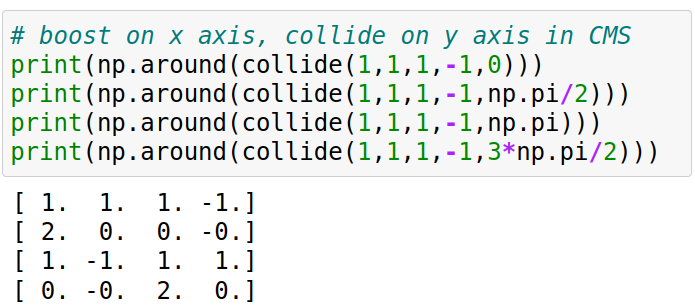
\includegraphics[width=0.65\textwidth]{figs/maxwellboltzman/collxy.png} \\
  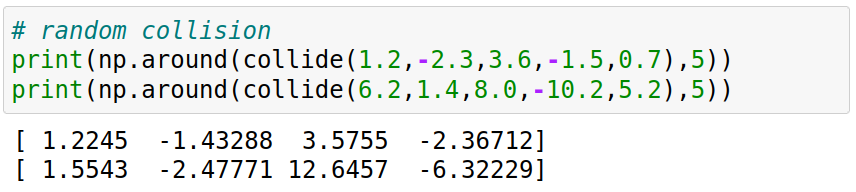
\includegraphics[width=0.65\textwidth]{figs/maxwellboltzman/collrand.png} \\
  \caption{More complicated example collisions.}
\label{fig:collcomp}
\end{center}
\end{figure}

\begin{plot} \end{plot}  Test your collision algorithm using the  example collisions from Fig.~\ref{fig:collcomp}.

\section{Initializing the Simulated Ideal Gas}

You will be modeling an ideal gas by direct Monte Carlo simulation of
{\tt NGAS} representative molecules.  We will use {\tt NGAS=1000}
intially, and you should use an even lower value while debugging.
We'll assume that the mass of each molecule in the gas is $M_0$,
or in the numerical system of units {\tt M=1}.

The state of your simulation will be completely contained in two numpy
arrays {\tt vx} and {\tt vy}, each of length {\tt NGAS}, which contain
the velocities of the particles in units of $V_0 = \sqrt{k_b T_0 /
  M_0}$.  Remember, the simulation uses a system of units that should
keep velocities near 1, so values such as 2.2, -3.1, 0.8, -0.01 are
all likely, and correspond to speeds up to several hundred meters per
second in SI units.  On the other hand, the presence of extremely
small values, like 5.3E-23, and extremely large values like 1.2E18 and
-8.2E28 are symptoms of bugs.

\begin{plot} Initialize both velocity arrays {\tt vx} and {\tt vy} of length {\tt NGAS}
with values choosen as uniform random variables in the range
$[-2,2]$. Fill two histograms, one with $v_x$ and one with $v_y$, with
an approriate range and 20 bins.  You should see that the velocities
are distributed uniformly (a flat distribution).  The distribution does not yet
resemble the Gaussian shape of Equation~\ref{eqn:mbvx} because it has not yet reached
thermal equilibrium.\end{plot}


\section{Collisions of an Ideal Gas}

To reach thermal equilibrium, you'll need to simulate collisions
betweens pairs of molecules in your gas.  For each collision, do the following:
\begin{itemize}
 \item Choose two molecules at random as particles $a$ and $b$. (See {\tt np.random.choice}.)
 \item Choose a random value $\theta$ uniformly in the range $[0,2\pi]$ (See {\tt np.random.uniform}.)
 \item Call your collision function with components of the velocity vectors for particles $a$ and $b$ and the scattering angle $\theta$.
 \item Update the velocity of particles $a$ and $b$ from the return value of your collision funciton
\end{itemize}   
For this model, you will need about 10 times as many collisions as gas
molecules in order to reach thermal equilibrium.

\begin{plot}  For {\tt NGAS=1000} simulate {\tt NCOLL = 10000} collisions as described above.
Fill two histograms, one with $v_x$ and one with $v_y$, with an
approriate range and 20 bins.  After reaching thermal equilibrium, the
distributions should resemble a Gaussian as predicted by Equation~\ref{eqn:mbvx}. \end{plot}

\section{Temperature of an Ideal Gas}

The temperature of the gas is related to the mean kinetic energy by:
\begin{equation}
\label{eqn:kt}
k_b T = m \, \frac{\braket{v_x^2} + \braket{v_y^2}}{2}  
\end{equation}  
You can estimate $\braket{v_x^2}$ from your simulation as {\tt np.mean(vx**2)}.

\begin{plot} Estimate $kT$ of the gas using Equation~\ref{eqn:kt} before and after simulating collisions.
The values should remain near the expected value 4/3.
\end{plot}

\section{The Maxwell-Boltzmann Distribution}

In this section, you'll reproduce the instructor plots of Fig.~\ref{fig:mbinst} using your own numerical simulation.

\begin{figure}[htbp]
\begin{center}
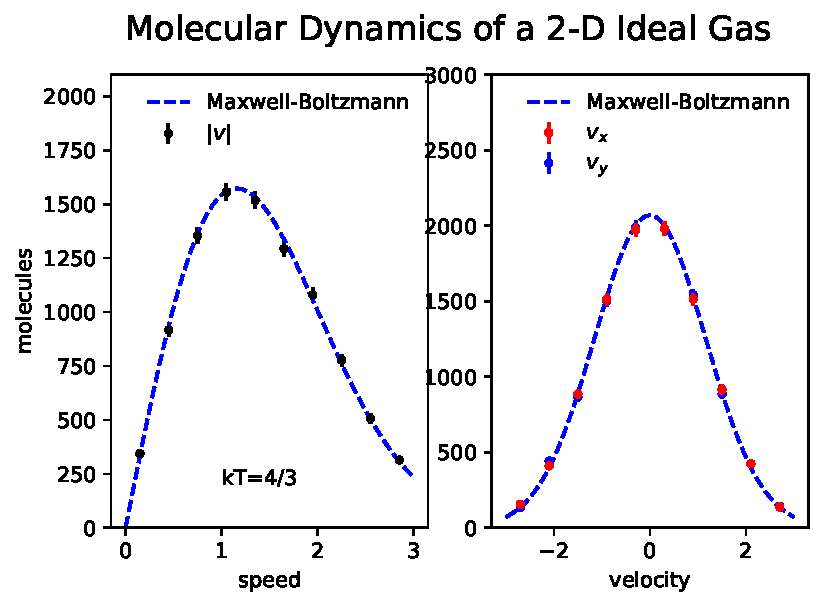
\includegraphics[width=0.85\textwidth]{figs/maxwellboltzman/maxboltz-instr.pdf} \\
\caption{Instructor plots.}
\label{fig:mbinst}
\end{center}
\end{figure}

\begin{plot}
  After your simulation reaches equilibrium, fill two histograms, one with $v_x$ and one with $v_y$, with an approriate range and 10 bins.  Compare with the prediction from Equation~\ref{eqn:mbvx}.  The results should resemble the right side of Fig.~\ref{fig:mbinst}, which were produced with {\tt NGAS=10000}.
\end{plot}

\begin{plot}
  After your simulation reaches equilibrium, fill a histograms with the magnitude of the velocity $v$, with an approriate range and 10 bins.  Compare with the prediction from Equation~\ref{eqn:mbv}.  The results should resemble the left side of Fig.~\ref{fig:mbinst}, which were produced with {\tt NGAS=10000}.
\end{plot}


  
